% Chapter 3
% Roberto Masocco <robmasocco@gmail.com>
% September 20, 2021

\chapter[Caso di studio: drone autonomo]{Caso di studio: drone autonomo}
\label{chap:Chapter3}
\doublespacing
\fontsize{14}{14}\selectfont
\indent A seguito della discussione portata a termine nei capitoli precedenti circa le nuove soluzioni hardware e software da impiegare per la costruzione di apparati robotici, verrà ora descritto un caso di studio pratico con cui si dimostreranno la validità e l'efficacia di tali strumenti: un drone volante automatico.\\
I task che tale sistema deve svolgere, oltre naturalmente a quelli inerenti il volo in sé, sono specificati nelle regole dell'edizione 2021 del Drone Contest indetto da Leonardo S.p.A. e tenutosi presso la Divisione Velivoli di Leonardo in Corso Francia, Torino. Il prototipo è stato presentato in tale occasione come la proposta del team Asgard Flight Group dell'Università di Roma "Tor Vergata". Il progetto ha coinvolto in tutto cinque tra tesisti e dottorandi afferenti al Dipartimento di Ingegneria Civile e Ingegneria Informatica, i quali sono citati all'inizio di questa Tesi assieme ai loro ruoli e ad un sentito e personale ringraziamento, sotto la supervisione del Prof. Daniele Carnevale. Le regole dell'edizione 2021 del Contest, che costituiscono gli obiettivi operativi del drone, possono essere riassunti come segue:
\begin{itemize}
    \item il drone deve essere in grado di decollare, volare e atterrare autonomamente, orientandosi all'interno di un ambiente indoor di cui è nota a priori la conformazione e la posizione delle piazzole di decollo e atterraggio;
    \item inizialmente il drone deve esplorare l'ambiente, cercando ed individuando dei target mobili costituiti da robot di tipo Roomba che montano un landmark ArUco;
    \item sono noti solo alcuni dei landmark montati sui robot, dunque quando il drone ne individuasse uno sconosciuto, dovrà scattare ed inviare delle fotografie di esso ad una \emph{Ground Control Station} controllata da un operatore;
    \item sulla base di una stringa di punteggi segnata vicino al landmark del robot, dovrà essere decisa una sequenza di atterraggi sulle varie piazzole;
    \item una volta trasmessa la sequenza al drone, esso dovrà eseguire i vari atterraggi, riconoscendo le piazzole sapendone la posizione nella mappa e rilevando i landmark ArUco dipinti su di esse;
    \item durante tutta la durata del volo deve essere possibile inserire il controllo manuale, per ragioni di sicurezza;
\end{itemize}
Per brevità sono stati tralasciati dei dettagli del regolamento inerenti il solo funzionamento della gara. L'obiettivo finale del Contest è chiaramente la massimizzazione del punteggio ottenuto con gli atterraggi, resa non banale dalla presenza nella mappa di ostacoli, rialzi e zone a bassa visibilità.\\
Nel resto di questo capitolo si descriverà più nel dettaglio il robot, partendo dall'hardware e passando poi al software, da quello di più basso livello fino alle logiche di supervisione e comunicazione con GCS ed operatori.\\
Il prototipo realizzato, assieme ad un esempio di landmark ArUco, sono ritratti in Figura \ref{fig:drone}.

\begin{figure}
    \centering
    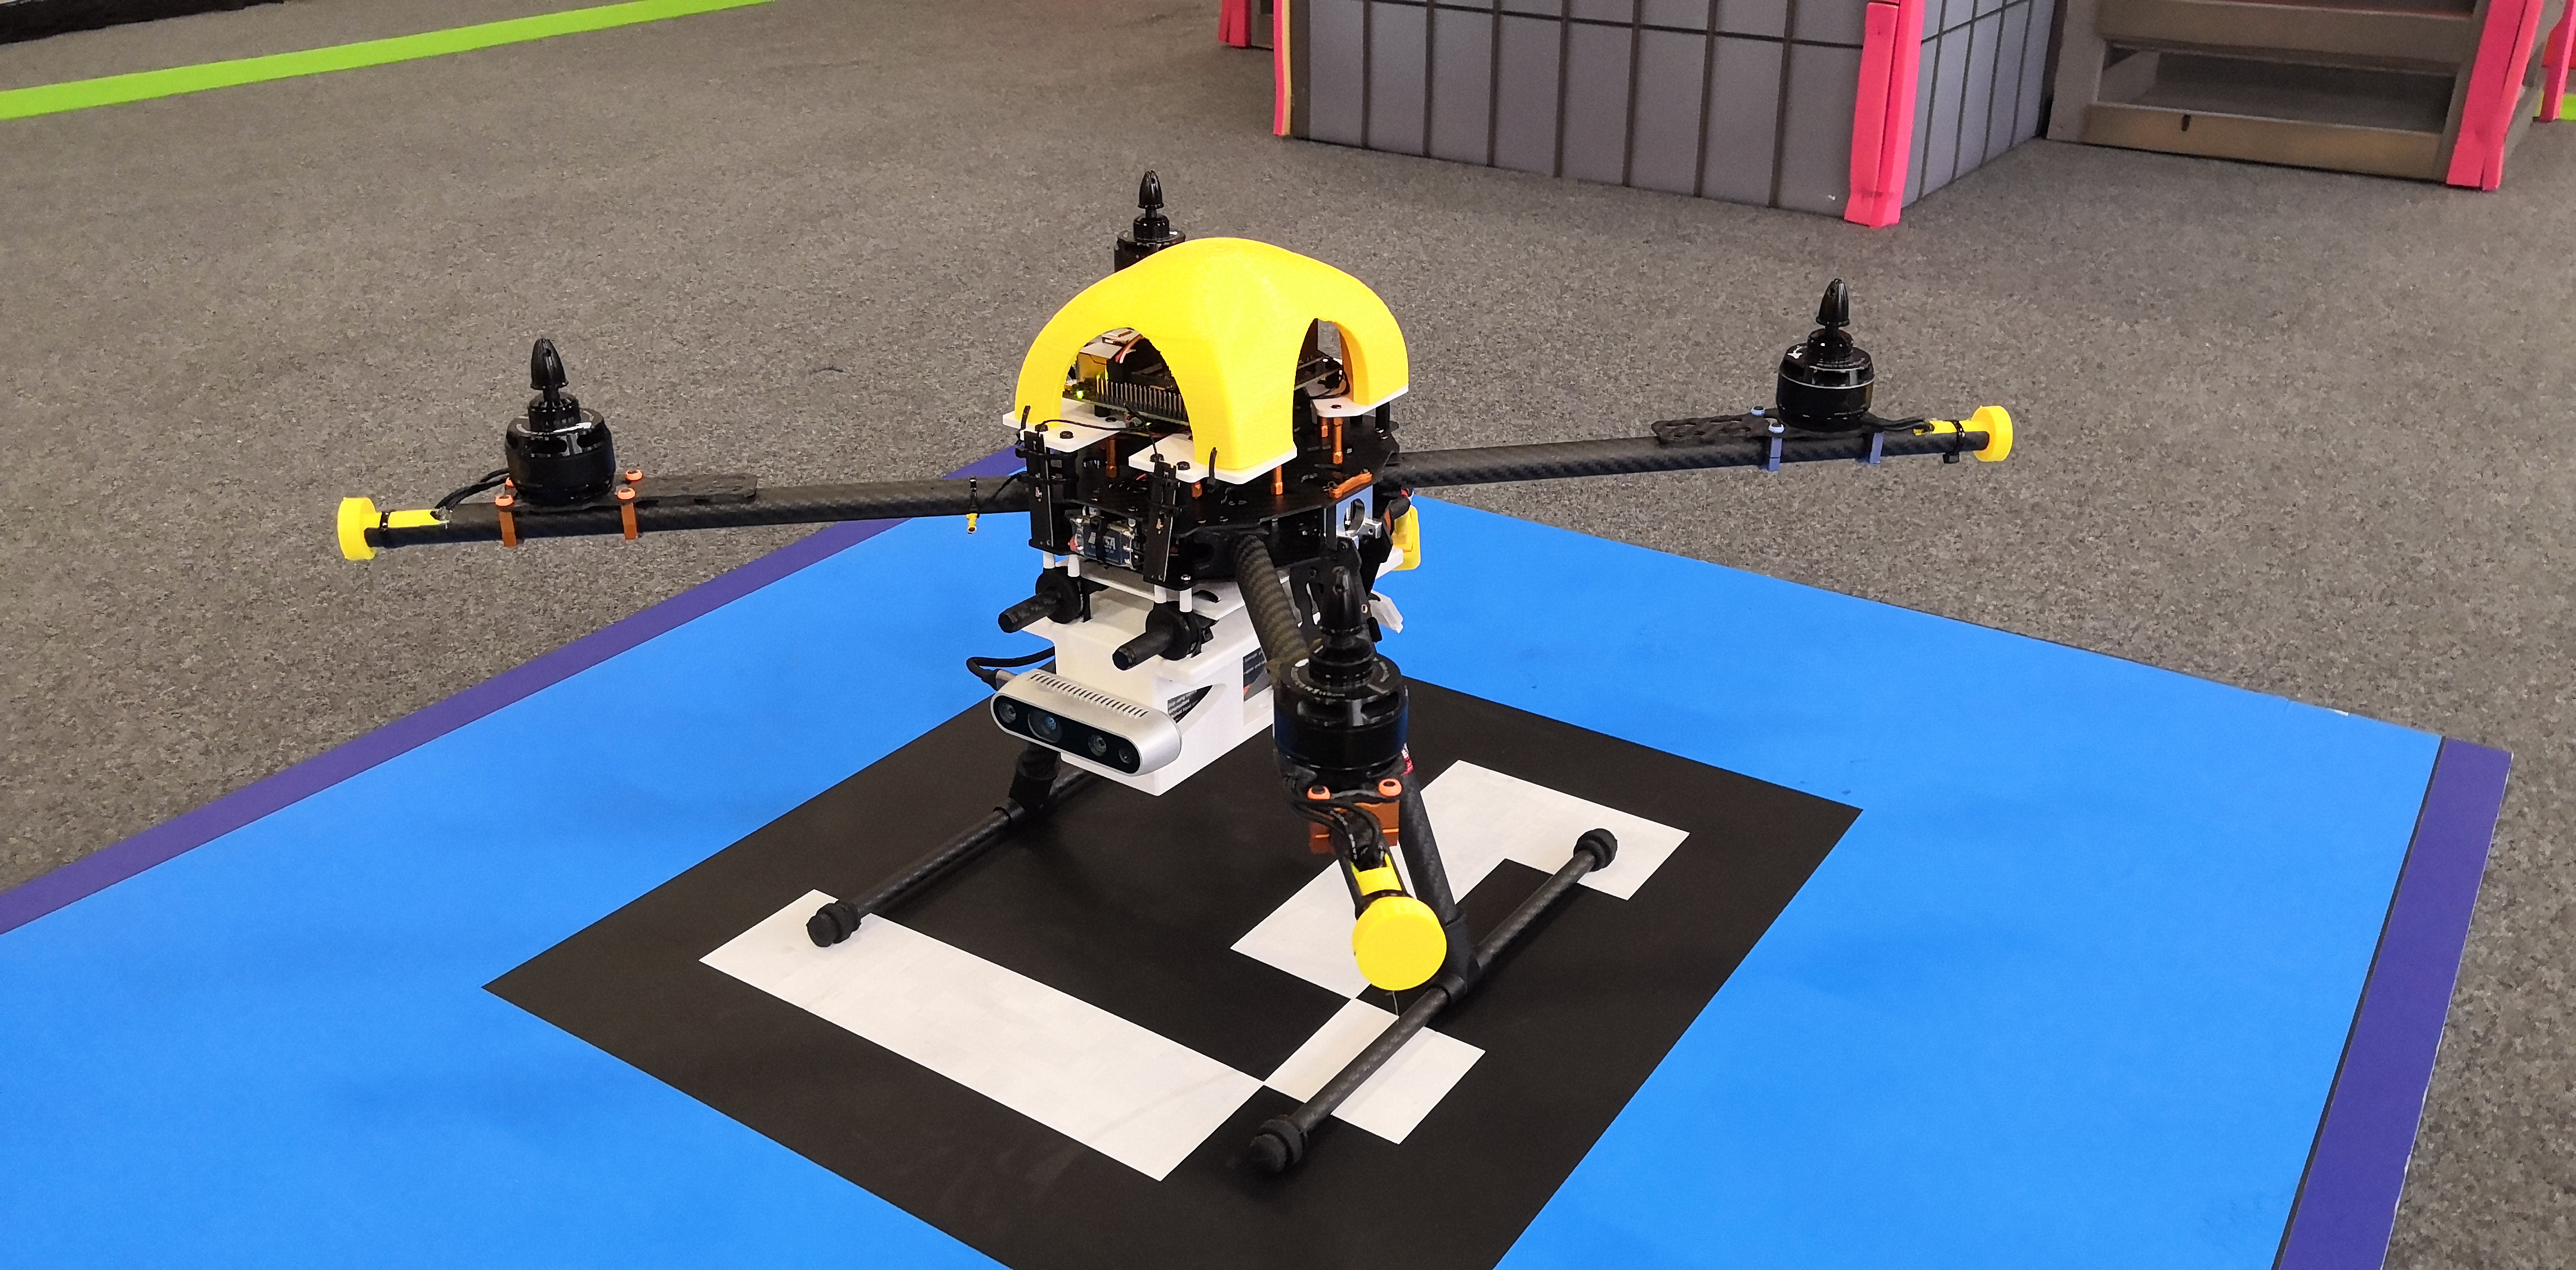
\includegraphics[width=0.9\textwidth]{figs/chapter3/drone_aruco.jpg}
    \caption{Prototipo del drone con le eliche rimosse su una piazzola del campo.}
    \label{fig:drone}
\end{figure}
\clearpage

\newsection{Hardware}
\indent

\newsection{Operating System}
\indent

\newsection{Software}
\indent

\newsection{Realizzazione}
\indent
